\newpage
\section{Complex Attribute Manipulation}
\visHeader
In Section~\ref{sec: Implementing check} we have modeled the \texttt{Partition::check()} method.
However, as you might realized, our implementation ignores the \texttt{partitionSize}, i.e., the maximal number of cards that fit in a partition.
In order to prevent our implementation from ``bursting" a partition we gonna use \emph{complex attribute constraints} to extend the SDM for the \texttt{Partition::check()} method. 
In contrast to simple attribute constrains\footnote{First used in Section~\ref{sec: Implementing check} to compare user’s guess against the card's face value}, which provide only binary operations for comparing attribute values (or literals), complex attribute constraints provides a language to specify arbitrary relations on attributes.

\subsection{Using Complex Attribute Constrains}     
We start by extending the \texttt{penalizeCard} pattern of the \texttt{Partition::check()} method in such a way that it only moves a card to the previous partition if the additional card does not exceed the actual \texttt{partitionSize} of the previous partition. But before we start we have to extend \texttt{Partition} class by an attribute that keeps track of the actual number of card contained in a partition:

\begin{figure}[htbp]
\begin{center}
  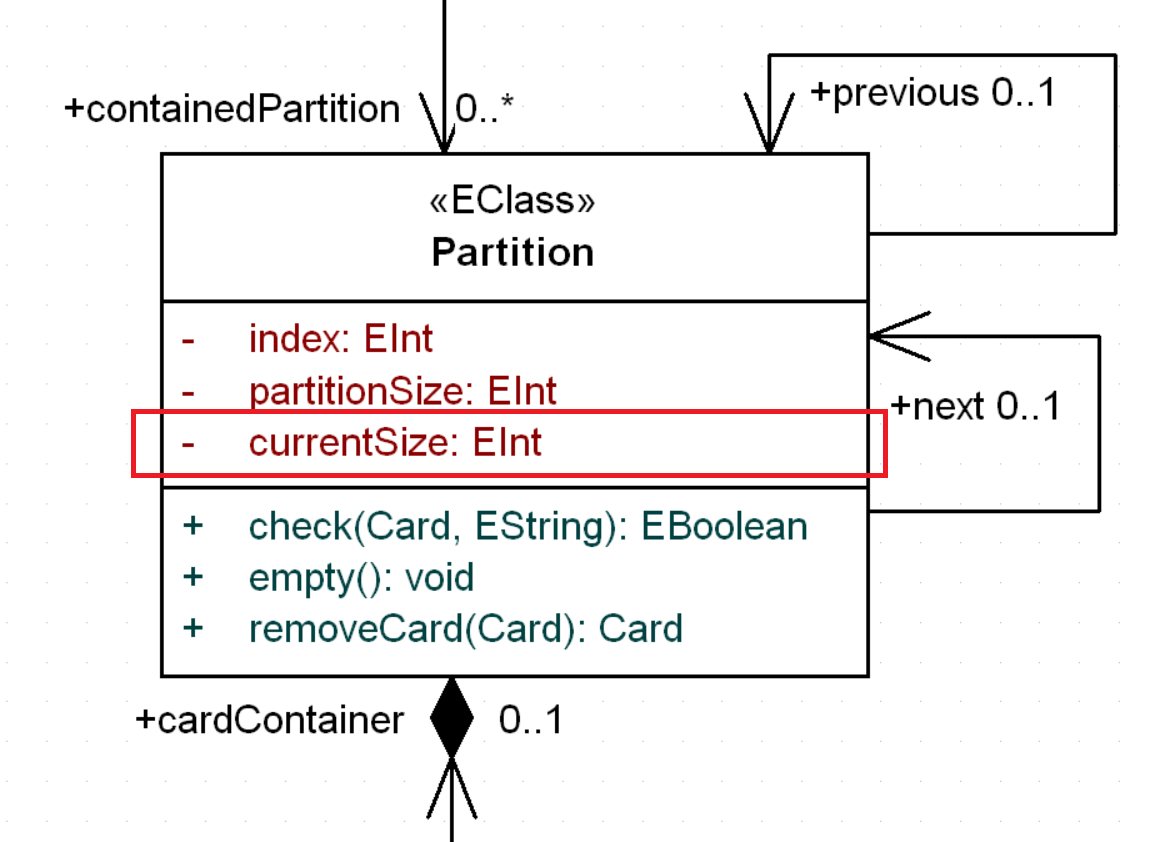
\includegraphics[width=0.8\textwidth]{ea_CAC_newAtributes}
  \caption{adding \texttt{currentSize:EInt} to \texttt{Partition}}  
  \label{ea_CAC_newAtributes}
\end{center}
\end{figure}

\begin{itemize}    
\item[$\blacktriangleright$] Add to the class \texttt{Partition} the new attribute \texttt{currentSize:EInt}.
\end{itemize} 

Now we can start defining complex attribute constraints:
\begin{figure}[htbp]
\begin{center}
  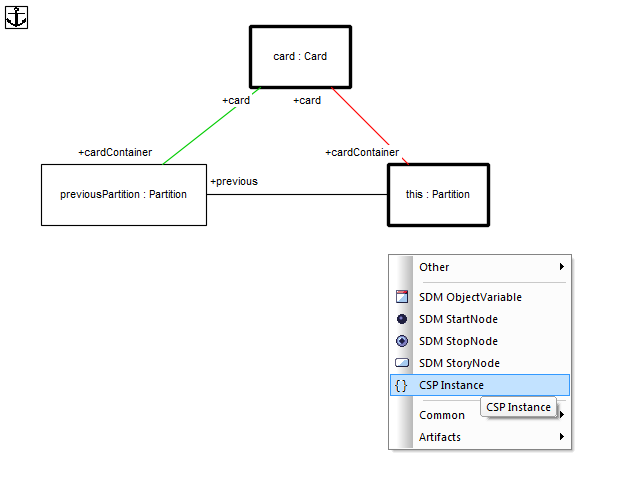
\includegraphics[width=0.8\textwidth]{ea_CAC_NewCSP}
  \caption{Creating a new \texttt{CSP instance}}  
  \label{ea:CAC_NewCSP}
\end{center}
\end{figure}
\begin{itemize}    

\item[$\blacktriangleright$] Navigate to the \texttt{penalizeCard} pattern in the \texttt{Partition::check()} method and add a \texttt{CSP instance};  
Following a similar process as creating a new object variable, i.e., either hit the spacebar or use the toolbox to create a new \emph{CSP instance} (Fig.~\ref{ea:CAC_NewCSP}).

\item[$\blacktriangleright$] You’ll notice a box were you can specify your complex attribute constraints. Enter the attribute constraints as shown in Fig.~\ref{ea:ea_CAC_DefineCSP} to define that a card is only moved if the additional card does not exceed the actual \texttt{partitionSize} of the previous partition.

\end{itemize}

Basically an attribute constraint is a predicate of the form

~~~~\texttt{SYMB(param$_1$,\ldots,param$_n$)}

\noindent consisting of an symbol \texttt{SYMB} naming the predicate, followed by a list of parameters. A parameter can be:
\begin{itemize}
    \item A \emph{local variables} of the form \\
    \hspace*{0.5cm} \texttt{varname:Type},\\
    as for example, \texttt{newPrevCurrentSize:EInt} (first line Fig.~\ref{ea:ea_CAC_DefineCSP})\\
     defines an local variable \texttt{newPrevCurrentSize} of type \texttt{EInt}. 
    \item A \emph{constant} is of the form \\
    \hspace*{0.5cm} \texttt{value:Type},\\
    as for example, \texttt{1:EInt} (first line Fig.~\ref{ea:ea_CAC_DefineCSP}) represents constant 1 of type \texttt{EInt}.
    \item An \emph{attribute variable} of the form \\
    \hspace*{0.5cm}\texttt{objectVarName.attributeName}, \\
     and refers to the current value of the attribute \texttt{attributeName} of object variable 	\texttt{objectVarName}, while an attribute variable of the form \texttt{objectVarName.attribteName'} refers to an attribute value after the transformation. This is necessary for, 	e.g., write the java expression \texttt{a.x=a.x+1} as the predicate \texttt{+(a.x', a.x, 1:EInt)}. 
\end{itemize}


 
\begin{figure}[htbp]
\begin{center}
  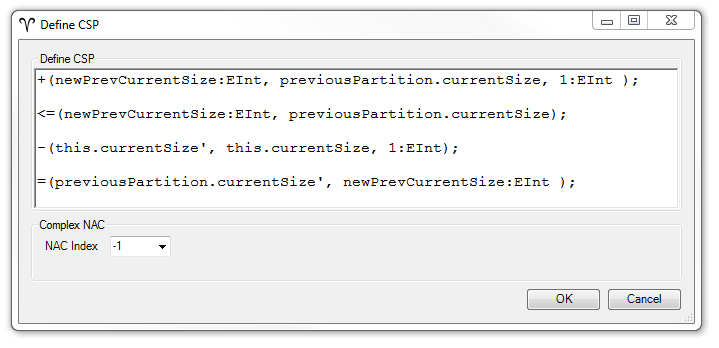
\includegraphics[width=0.99\textwidth]{ea_CAC_DefineCSP}
  \caption{Defining complex attribute constraints}  
  \label{ea:ea_CAC_DefineCSP}
\end{center}
\end{figure}

The \texttt{CSP instance} (the set of attribute constraints) shown in Fig.~\ref{ea:ea_CAC_DefineCSP} consist of the constraints with meaning \footnote{An complete list of build in constraints is given at the end of this chapter.}:

\hspace*{0.5cm}\texttt{\small +(newPrevCurrentSize:EInt, previousPartition.currentSize, 1:EInt)},\\
meaning that:\\
\hspace*{0.5cm}\texttt{\small newPrevCurrentSize == previousPartition.currentSize + 1};

\hspace*{0.5cm}\texttt{\small<=(newPrevCurrentSize:EInt, previousPartition.currentSize)},\\
meaning that:\\
\hspace*{0.5cm} \texttt{\small newPrevCurrentSize $\leq$ previousPartition.currentSize};

\hspace*{0.5cm}\texttt{\small-(this.currentSize', this.currentSize, 1:EInt)},\\
meaning that:\\
\hspace*{0.5cm} \texttt{\small this.currentSize' == this.currentSize - 1};

\hspace*{0.5cm}\texttt{\small=(previousPartition.currentSize', newPrevCurrentSize:EInt)},\\
meaning that:\\
\hspace*{0.5cm} \texttt{\small previousPartition.currentSize' == newPrevCurrentSize}.
\begin{itemize}    
\item[$\blacktriangleright$] Export the project as usual. Before you start generating code you have to switch the code generation engine. Open the \texttt{moflon.properties.xmi} located in your project and change the \textsf{SDM Codegenerator Method Body Handler} to  \textsf{DEMOCLES\_ATTRIBUTES} (Fig.~\ref{ec_CAC_SwitchCGE}).

\begin{figure}[htbp]
\begin{center}
  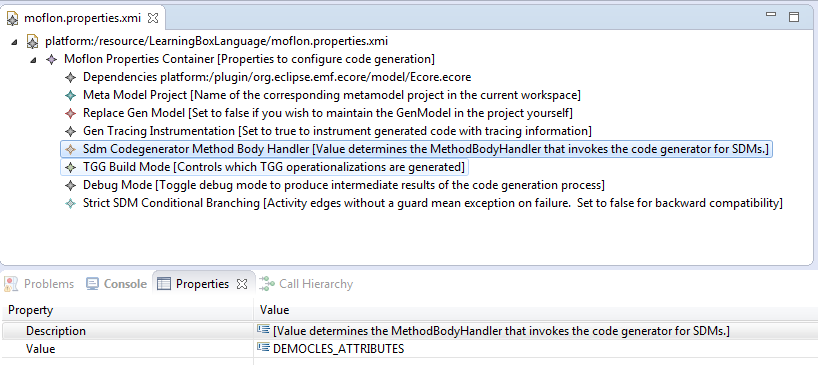
\includegraphics[width=0.99\textwidth]{ec_CAC_SwitchCGE}
  \caption{Switch \textsf{SDM Codegenerator Method Body Handler} to \textsf{DEMOCLES\_ATTRIBUTES}}  
  \label{ec_CAC_SwitchCGE}
\end{center}
\end{figure}

\end{itemize}
The code generator engine is now able to solve the CSP instances, i.e., the constraints are operationalized and put in correct order. 
The code resulting for the CSP instance is shown in Figs.~\ref{ea_CAC_penalizeCardLHS} and \ref{ea_CAC_penalizeCardRHS} for the LHS and RHS, respectively.
\begin{figure}[htbp]
\begin{center}
  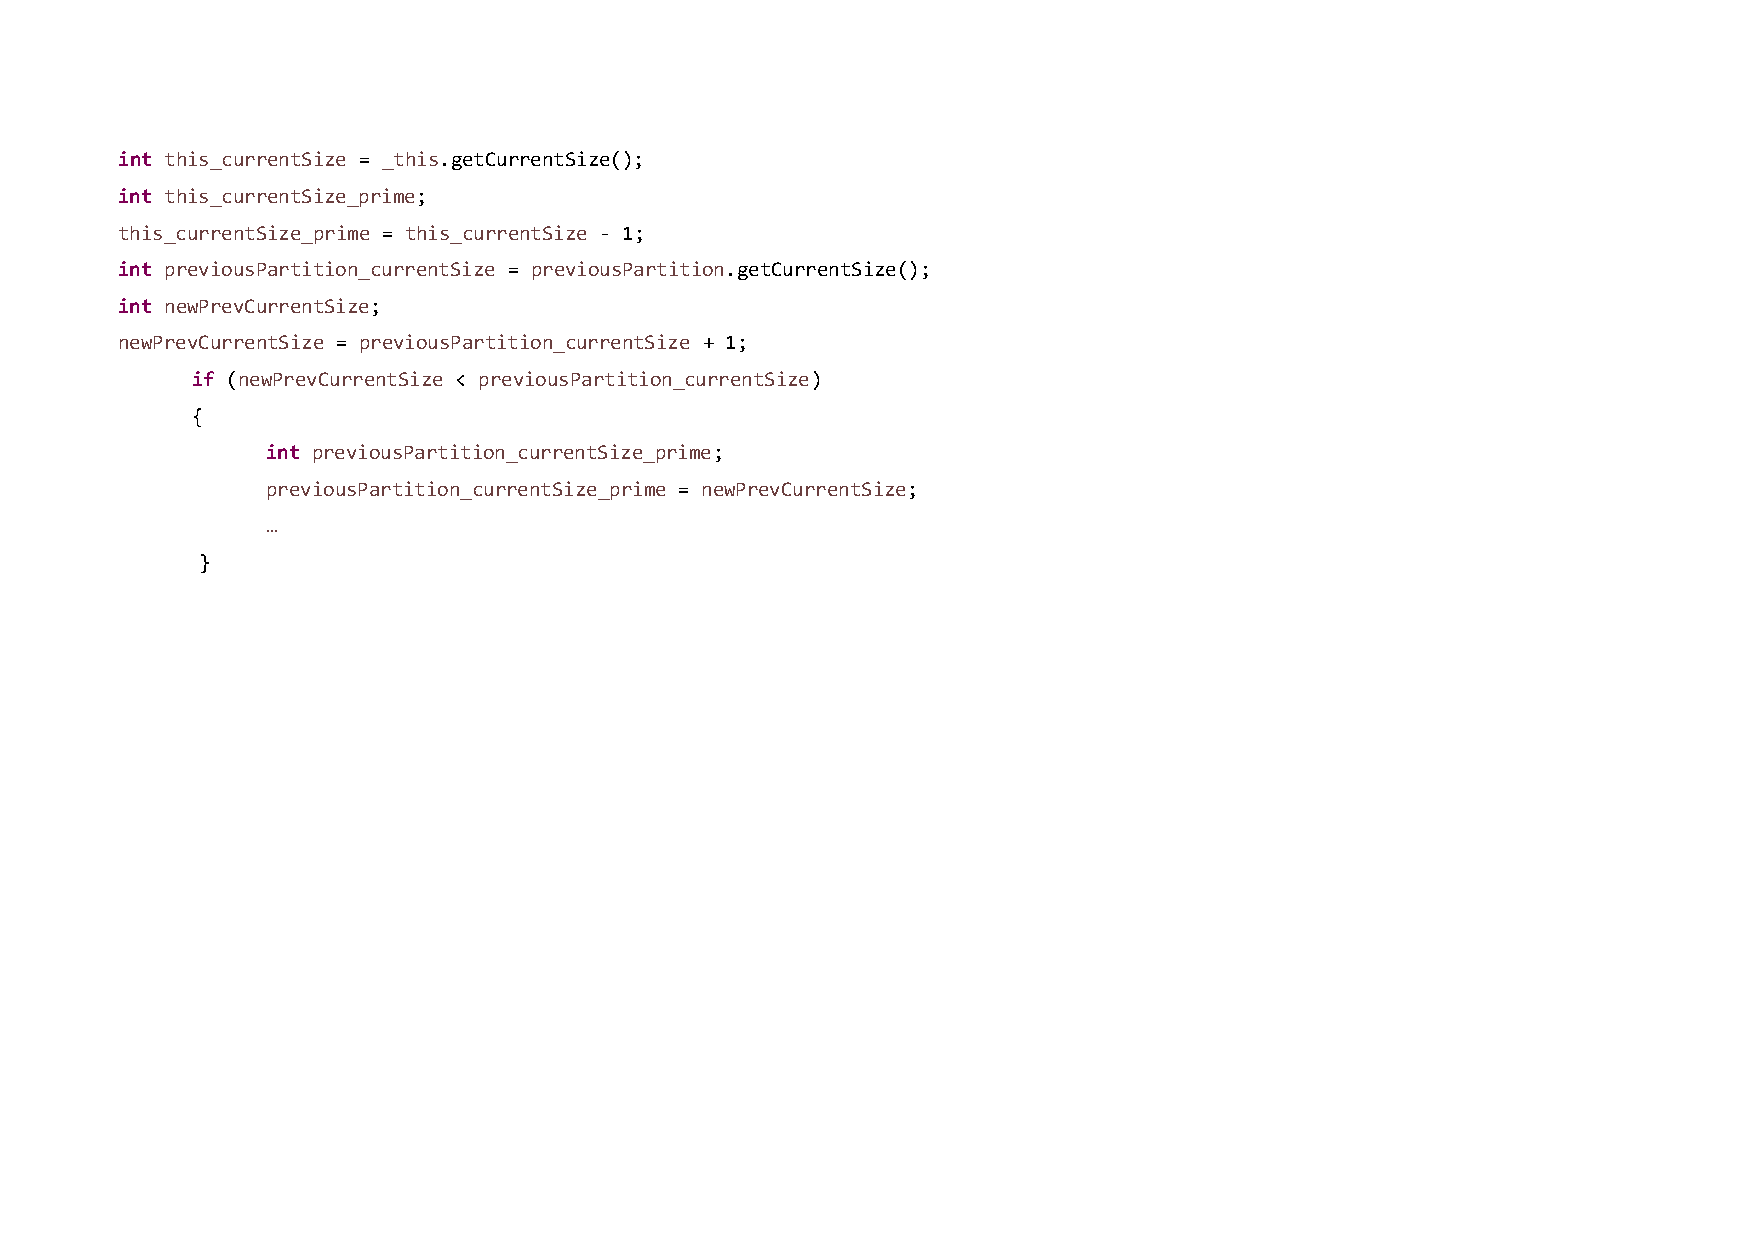
\includegraphics[width=0.99\textwidth]{ea_CAC_penalizeCardLHS.pdf}
  \caption{LHS pattern code generated for the CSP instance}  
  \label{ea_CAC_penalizeCardLHS}
\end{center}
\end{figure}
\begin{figure}[htbp]
\begin{center}
  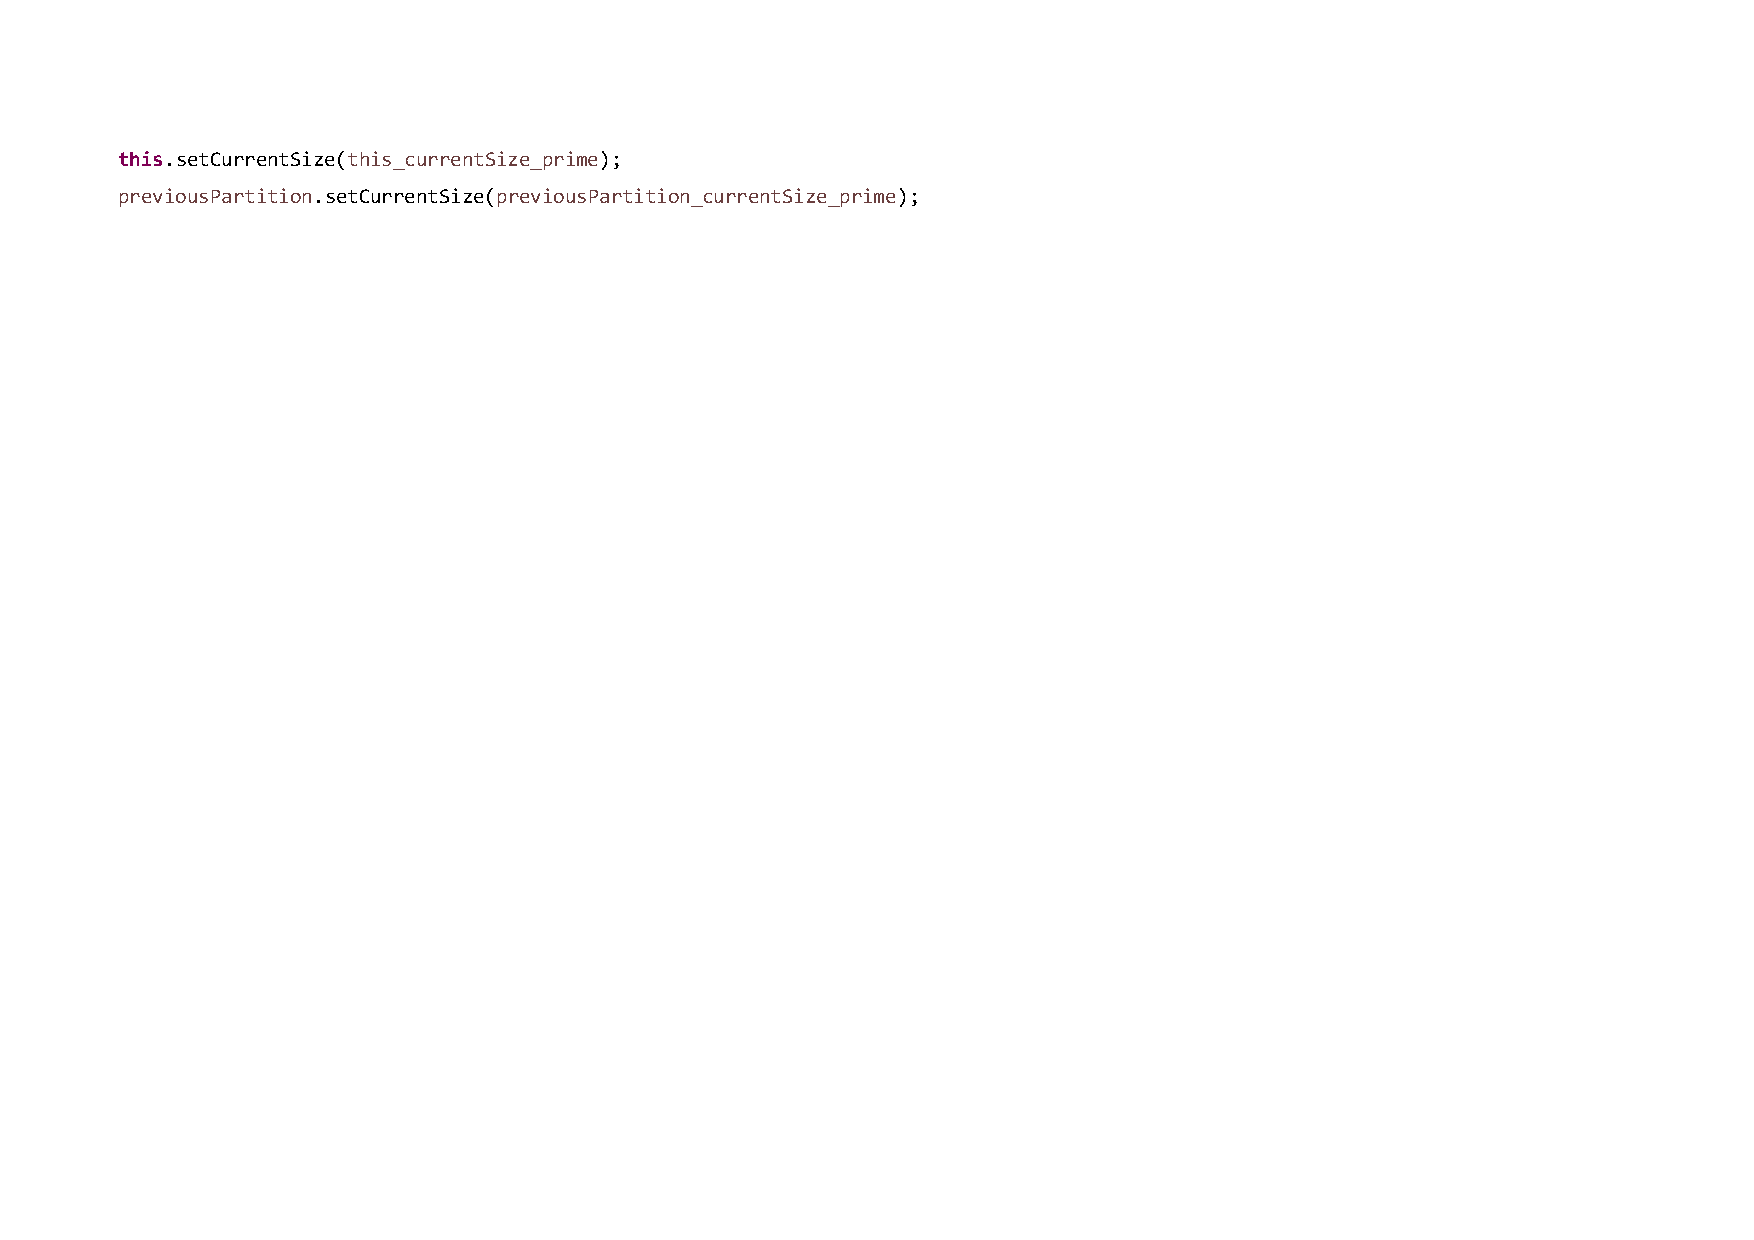
\includegraphics[width=0.99\textwidth]{ea_CAC_penalizeCardRHS.pdf}
  \caption{RHS pattern code generated for the CSP instance}  
  \label{ea_CAC_penalizeCardRHS}
\end{center}
\end{figure}

Notice that the attribute variables \texttt{this.currentSize'} and \\
\texttt{previousPartition.currentSize'} (represented in the code by \\ 
\texttt{this\_currentSize\_prime} and \texttt{previousPartition\_currentSize\_prime}, respectively) are treated as local variables on the LHS and then assigned on the RHS to the corresponding attribute values.
Hence we might rewrite the \texttt{CSP instance} shown in Fig.~\ref{ea:ea_CAC_DefineCSP} to the more compact shown in Fig.\ref{ea:ea_CAC_DefineCSP2}.
\begin{figure}[htbp]
\begin{center}
  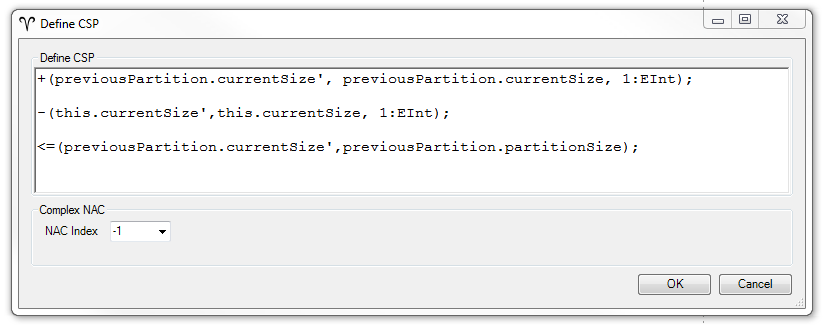
\includegraphics[width=0.99\textwidth]{ea_CAC_DefineCSP2}
  \caption{Defining complex attribute constraints}  
  \label{ea:ea_CAC_DefineCSP2}
\end{center}
\end{figure}

\subsection{Defining Own Complex Attribute Constraints}  
In Section~\ref{sec_A string representation of our learning box} we have implemented the \texttt{Box::toString()} method to obtain a string representation of the box. 
The method uses internally the method \texttt{Box::addToStringRep(Card) : EString} to create a string from a card, that was realized using handwritten code via injections.

In the following the \texttt{Box::addToStringRep(Card):EString} method should be replaced by using complex attribute constraints.

\begin{itemize}
  \item[$\blacktriangleright$] Reconsider the SDM shown in Fig.~\ref{ea:sdm_tostringComplete}. First add an attribute constraint for appending the string \texttt{"PartitionContent:"} to the \texttt{stringRep} attribute of \texttt{ Box}. To this end, add to the \texttt{ForAllPartitons} pattern the complex attribute constraint:\\
\hspace*{0.5cm} \texttt{\small +(this.stringRep',this.stringRep, "Partition Content:":EString)},\\
\end{itemize}  
Note that the ``+'' predicate is overloaded, while \texttt{\small +( :EInt, :EInt, :EInt)} (as used in the previous section), means integer addition, \\
  \texttt{\small +( :EString, :EString, :EString)} is concatenation.
   	  


In a next step the \emph{ForAllCards} pattern should be extended by an complex attribute constraints such that for each card the string containing the front and back is appended to \emph{this.stringRep}.  	 
Instead of using the the concat (\texttt{+}) operation again, we just cand to define our own constraint by
\begin{itemize}
\item[$\blacktriangleright$] just adding the \texttt{CSP instance}: \\
\hspace*{0.5cm}\texttt{\small myConcat(this.stringRep', this.stringRep, card.face, card.back)}\\
to the \texttt{ForAllCards} pattern. The complete SDM should now look as shown in Fig.~\ref{ea_CAC_CompletToString}.

\begin{figure}[htbp]
\begin{center}
  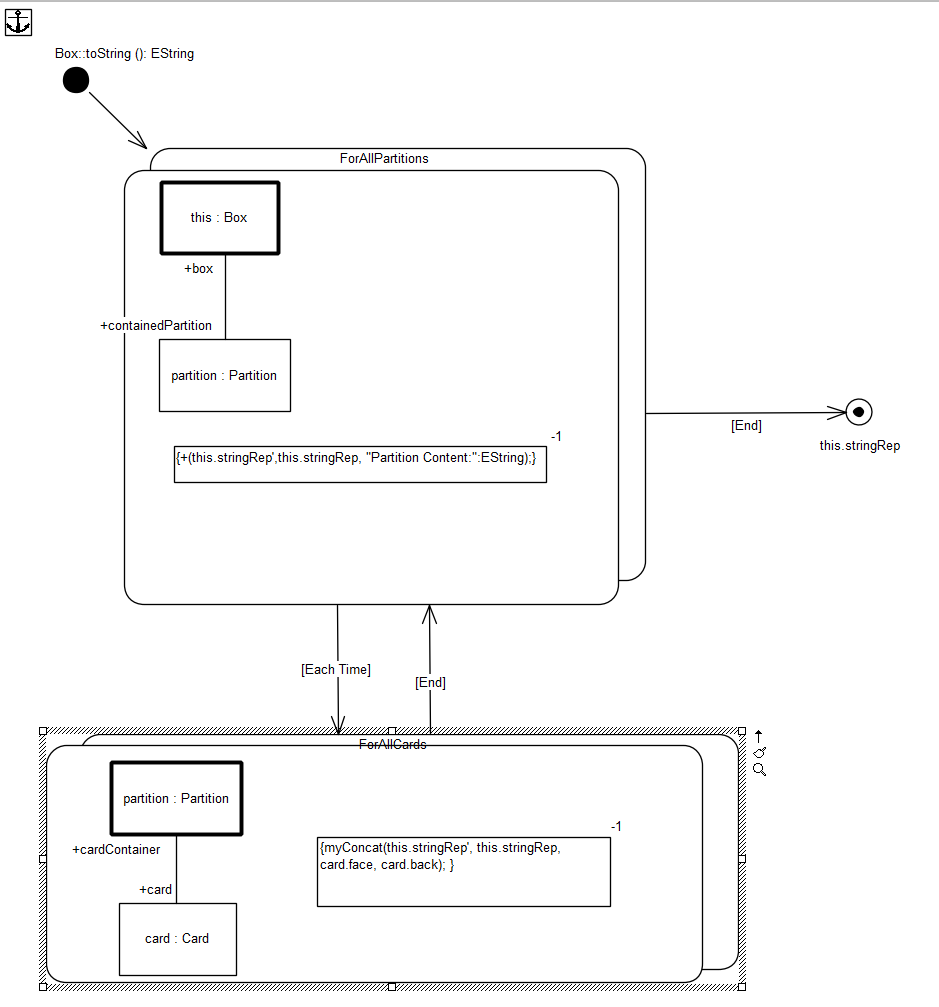
\includegraphics[width=0.99\textwidth]{ea_CAC_CompletToString}
  \caption{Complet SDM for \texttt{Box::toString()}}  
  \label{ea_CAC_CompletToString}
\end{center}
\end{figure}
\item[$\blacktriangleright$] Export as usual. If you are trying to build the metamodel project in eclipse you get an error message (Fig.~\ref{ec_CAC_Malformed}) that informs you that the attribute constraint with signature: \\
\hspace*{0.5cm} \texttt{\small myConcat( :EString, :EString, :EString, :EString)} \\
is unknown. If you look at \texttt{LearningBoxLanguage/lib/} there is a new file  \texttt{LearningBoxLanguageAttributeConstraintsLib.xmi} 
 
\begin{figure}[htbp]
\begin{center}
  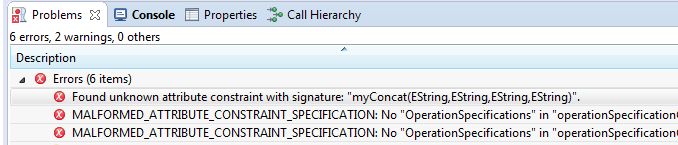
\includegraphics[width=0.99\textwidth]{ec_CAC_Malformed}
  \caption{Error}  
  \label{ec_CAC_Malformed}
\end{center}
\end{figure}



\item[$\blacktriangleright$] Open the file. It contains a constraint specification \texttt{myConcat} (Fig.\ref{ec_CAC_lib} bottom) that represents the signature (\texttt{\small myConcat( :EString, :EString, :EString, :EString)}) which is derived from the information of the CSP-instance in EA. To define the meaning of \texttt{myConcat} we have to define operations for the constraint.

\begin{figure}[htbp]
\begin{center}
  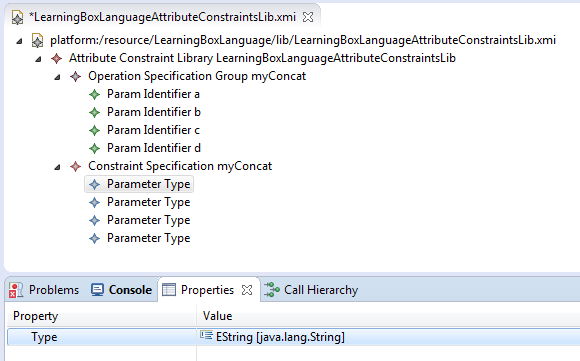
\includegraphics[width=0.95\textwidth]{ec_CAC_lib}
  \caption{The content of LearningBoxLanguageAttributeConstraintsLib.xmi}  
  \label{ec_CAC_lib}
\end{center}
\end{figure}
\item[$\blacktriangleright$] Right click the operation specification group for \texttt{myConcat} (top of Fig.~\ref{ec_CAC_lib}) and add as new child an \texttt{operation specification}. 
\end{itemize}

An operation\footnote{Double click on the operation specification to open the properties view.} is specified by an \emph{Adornment String}, and a \texttt{Specification} that is a template defining the code to be generated.

\begin{figure}[htbp]
\begin{center}
  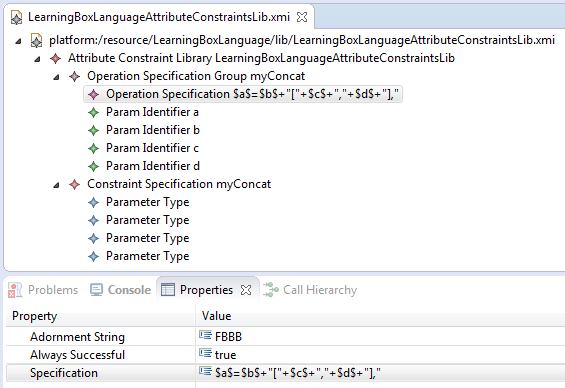
\includegraphics[width=0.99\textwidth]{ea_CAC_opSpec}
  \caption{The operation specification for myConcat}  
  \label{ea_CAC_opSpec}
\end{center}
\end{figure}

\begin{itemize}
\item[$\blacktriangleright$] Complete the operation specification as shown in Fig.\ref{ea_CAC_opSpec}. The adornment string \texttt{FBBB} means that before the operation can be executed the values for parameter 2--4 must be known (\texttt{B}ound), and the \texttt{F}ree parameter (i.e., the first parameter in this case) is derived from the \texttt{B}ound parameters. The \emph{Specification} field contains the template string that specifies a java expression that defines how the \texttt{F}ree parameter is derived from the \texttt{B}ound ones. The template uses the parameter identifier as variables (sounded with \$ \$). 

\end{itemize}



\goodbreak
 
\subsection{Build in Complex Attribute Constraints}  
\begin{table}[h]
\begin{center}
\begin{tabular}{| c| l | r |} \hline 
Symbol & Signatures  & Semantics \\ \hline \hline 
$=$ & (a:Eint , b:EInt) & $(a=b)$ \\ 
 & (a:EDouble , b:EDouble) & \\ 
 & (a:EFloat , b:EFloat) &  \\ 
 & (a:EShort , b:EShort) & \\ 
 & (a:ELong , b:ELong) &  \\ 
 & (a:EString , b:EString) & \\\hline
 $<=$ & (a:Eint , b:EInt) & $(a\leq b)$ \\ 
 & (a:EDouble , b:EDouble) & \\ 
 & (a:EFloat , b:EFloat) &  \\ 
 & (a:EShort , b:EShort) & \\ 
 & (a:ELong , b:ELong) &  \\\hline
 $<$ & (a:Eint , b:EInt) & $(a < b)$ \\ 
 & (a:EDouble , b:EDouble) & \\ 
 & (a:EFloat , b:EFloat) &  \\ 
 & (a:EShort , b:EShort) & \\ 
 & (a:ELong , b:ELong) &  \\\hline
 $>=$ & (a:Eint , b:EInt) & $(a\geq b)$ \\ 
 & (a:EDouble , b:EDouble) & \\ 
 & (a:EFloat , b:EFloat) &  \\ 
 & (a:EShort , b:EShort) & \\ 
 & (a:ELong , b:ELong) &  \\\hline
 $>$ & (a:Eint , b:EInt) & $(a > b)$ \\ 
 & (a:EDouble , b:EDouble) & \\ 
 & (a:EFloat , b:EFloat) &  \\ 
 & (a:EShort , b:EShort) & \\ 
 & (a:ELong , b:ELong) &  \\\hline
  \end{tabular}
  \end{center}
 \end{table} 
 \begin{table}[h]
\begin{center}
 \begin{tabular}{| c| l | r |} \hline 
Symbol & Signatures  & Semantics \\ \hline \hline  
$+$ & (a:Eint , b:EInt, c:EInt) & $(a=b+c)$ \\ 
 & (a:EDouble , b:EDouble, c:EDouble) & \\ 
 & (a:EFloat , b:EFloat, c:EFloat) &  \\ 
 & (a:EShort , b:EShort, c:EShort) & \\ 
 & (a: , b:, c:) & \\
 & (a:ELong , b:ELong, c:ELong) &  \\ 
 & (a:EString , b:EString, c:EString) & \\\hline
$-$ & (a:Eint , b:EInt, c:EInt) & $(a=b-c)$ \\ 
 & (a:EDouble , b:EDouble, c:EDouble) & \\ 
 & (a:EFloat , b:EFloat, c:EFloat) &  \\ 
 & (a:EShort , b:EShort, c:EShort) & \\ 
 & (a:ELong , b:ELong, c:ELong) &  \\ \hline
$ /$ & (a:Eint , b:EInt, c:EInt) & $(a=b/c)$ \\ 
 & (a:EDouble , b:EDouble, c:EDouble) & \\ 
 & (a:EFloat , b:EFloat, c:EFloat) &  \\ 
 & (a:EShort , b:EShort, c:EShort) & \\ 
 & (a:ELong , b:ELong, c:ELong) &  \\ \hline
$ *$ & (a:Eint , b:EInt, c:EInt) & $(a=b\cdot c)$ \\ 
 & (a:EDouble , b:EDouble, c:EDouble) & \\ 
 & (a:EFloat , b:EFloat, c:EFloat) &  \\ 
 & (a:EShort , b:EShort, c:EShort) & \\ 
 & (a:ELong , b:ELong, c:ELong) &  \\ \hline
  \end{tabular}
  \end{center}
 \end{table} 





   
